\begin{remark*}[Exposition]
Open and closed sets describe how subsets sit inside a metric space.  The
primitive local objects are open balls: a set is open when every one of its
points has a small ball that remains inside the set.  Closed sets are then
defined by open complements, and closure, interior, and boundary record the
points forced by these local tests.
\end{remark*}

\begin{definitionbox}{Definition --- Metric Open Set}
\begin{definition}[Metric Open Set]\label{def:metric-open-set}
Let \((X,d)\) be a metric space.  A subset \(E\subseteq X\) is \emph{open in
\((X,d)\)} if either \(E=\varnothing\) or, for every \(x\in E\), there exists
\(\varepsilon>0\) such that
\[
  B_d(x;\varepsilon)\subseteq E.
\]
\end{definition}
\end{definitionbox}

\begin{remark*}[Standard quantified statement]
\[
E\text{ is open in }(X,d)
\quad\Longleftrightarrow\quad
E\subseteq X
\;\land\;
\bigl(E=\varnothing
\;\lor\;
\forall x\in E\,\exists\varepsilon>0{:}\ B_d(x;\varepsilon)\subseteq E\bigr).
\]
\end{remark*}

\begin{remark*}[Interpretation]
An open set contains room around each of its points.  The amount of room may
depend on the point, but every point of the set must have some positive-radius
ball that stays inside the set.
\end{remark*}

\begin{remark*}[Examples]
In \(\mathbb{R}\) with the usual metric, each interval \((a,b)\) is open.
The interval \([a,b]\) is not open when \(a<b\), because the endpoints have no
positive-radius open interval contained in \([a,b]\).
\end{remark*}

\begin{figure}[htbp]
\centering
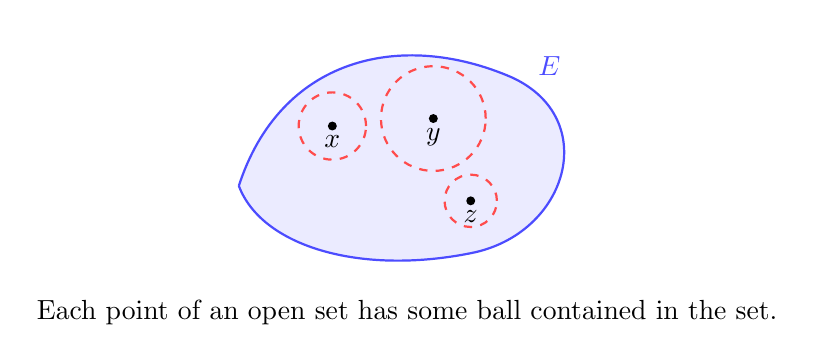
\begin{tikzpicture}[scale=0.95,>=stealth]
  \fill[blue!8]
    (-2.25,-0.45) .. controls (-1.7,1.25) and (-0.1,1.65) .. (1.4,1.0)
    .. controls (2.6,0.45) and (2.15,-1.1) .. (0.85,-1.35)
    .. controls (-0.65,-1.65) and (-1.95,-1.25) .. (-2.25,-0.45);
  \draw[blue!70,thick]
    (-2.25,-0.45) .. controls (-1.7,1.25) and (-0.1,1.65) .. (1.4,1.0)
    .. controls (2.6,0.45) and (2.15,-1.1) .. (0.85,-1.35)
    .. controls (-0.65,-1.65) and (-1.95,-1.25) .. (-2.25,-0.45);
  \node[blue!70] at (1.9,1.15) {\(E\)};

  \foreach \p/\r/\lab in {(-1.0,0.35)/0.45/x,(0.35,0.45)/0.7/y,(0.85,-0.65)/0.35/z}
  {
    \fill[black] \p circle (1.7pt);
    \node[below] at \p {\(\lab\)};
    \draw[red!70,thick,dashed] \p circle (\r);
  }

  \node[align=center] at (0,-2.15)
    {Each point of an open set has some ball contained in the set.};
\end{tikzpicture}

\caption{Openness is a local condition: every point of an open set has some
positive-radius ball contained in the set.}
\label{fig:open-set-local-room}
\end{figure}

\begin{dependencies}
\begin{itemize}
  \item \hyperref[def:metric-space]{Definition: Metric Space}
  \item \hyperref[def:metric-open-ball]{Definition: Open Ball}
\end{itemize}
\end{dependencies}

\begin{theorembox}{Theorem}
\begin{theorem}[Open Balls are Open]
\label{thm:metric-open-balls-are-open}
Let \((X,d)\) be a metric space.  For every \(x\in X\) and every \(r>0\),
the open ball \(B_d(x;r)\) is open in \((X,d)\).

\smallskip
\noindent
\hyperref[prf:metric-open-balls-are-open]{\textit{Go to proof.}}
\end{theorem}
\end{theorembox}

\begin{remark*}[Standard quantified statement]
\[
\forall x\in X\,\forall r>0{:}\quad
B_d(x;r)\text{ is open in }(X,d).
\]
\end{remark*}

\begin{remark*}[Predicate reading]
\[
\operatorname{IsBall}(B_d(x;r),x,r,(X,d))
\Longrightarrow
\operatorname{IsOpen}(B_d(x;r),(X,d))
\]
means that every open ball is an open subset of its metric space.
\end{remark*}

\begin{remark*}[Interpretation]
Every metric ball contains room around each of its points.  The triangle
inequality is the mechanism that transfers room around the center to room
around an arbitrary point inside the ball.
\end{remark*}

\begin{remark*}[Historical note]
This result corresponds to Theorem~3.4 in Kainth's
\emph{A Comprehensive Textbook on Metric Spaces}
\cite{KainthComprehensiveMetricSpaces2023}.
\end{remark*}

\begin{dependencies}
\begin{itemize}
  \item \hyperref[def:metric-space]{Definition: Metric Space}
  \item \hyperref[def:metric-open-ball]{Definition: Open Ball}
  \item \hyperref[def:metric-open-set]{Definition: Metric Open Set}
  \item \hyperref[lem:metric-key-local-ball]{Lemma: Key Local Ball Lemma}
\end{itemize}
\end{dependencies}

\begin{theorembox}{Theorem}
\begin{theorem}[Metric Open Set Closure Properties]
\label{thm:metric-open-set-closure-properties}
Let \(X\) be a metric space.  Then:
\begin{enumerate}
  \item the empty set \(\varnothing\) and the space \(X\) are open sets;
  \item an arbitrary union of open subsets of \(X\) is open;
  \item any finite intersection of open subsets of \(X\) is open.
\end{enumerate}

\smallskip
\noindent
\hyperref[prf:metric-open-set-closure-properties]{\textit{Go to proof.}}
\end{theorem}
\end{theorembox}

\begin{remark*}[Standard quantified statement]
If \(X\) is a metric space, then
\[
\varnothing\text{ is open in }X,
\qquad
X\text{ is open in }X,
\]
\[
\{U_\alpha\}_{\alpha\in A}\text{ open in }X
\Longrightarrow
\bigcup_{\alpha\in A}U_\alpha\text{ is open in }X,
\]
and, for \(n\in\mathbb{N}\),
\[
U_1,\ldots,U_n\text{ open in }X
\Longrightarrow
\bigcap_{k=1}^{n}U_k\text{ is open in }X.
\]
\end{remark*}

\begin{remark*}[Interpretation]
Metric open sets are stable under the same basic operations that define a
topology: arbitrary unions and finite intersections.  Thus every metric
determines a topology by declaring its metric-open subsets to be open.
\end{remark*}

\begin{remark*}[Historical note]
This result corresponds to Theorem~3.2 in Kainth's
\emph{A Comprehensive Textbook on Metric Spaces}
\cite{KainthComprehensiveMetricSpaces2023}.
\end{remark*}

\begin{dependencies}
\begin{itemize}
  \item \hyperref[def:metric-space]{Definition: Metric Space}
  \item \hyperref[def:metric-open-set]{Definition: Metric Open Set}
\end{itemize}
\end{dependencies}

\begin{definitionbox}{Definition --- Metric Closed Set}
\begin{definition}[Metric Closed Set]\label{def:metric-closed-set}
Let \((X,d)\) be a metric space.  A subset \(E\subseteq X\) is \emph{closed in
\((X,d)\)} if its complement \(E^c=X\setminus E\) is open in \((X,d)\).
\end{definition}
\end{definitionbox}

\begin{remark*}[Standard quantified statement]
\[
E\text{ is closed in }(X,d)
\quad\Longleftrightarrow\quad
E\subseteq X
\;\land\;
E^c=X\setminus E
\;\land\;
E^c\text{ is open in }(X,d).
\]
\end{remark*}

\begin{remark*}[Interpretation]
A closed set is defined by the openness of what lies outside it.  In metric
spaces this means every point outside \(E\) has some positive-radius ball that
misses \(E\).
\end{remark*}

\begin{remark*}[Notation]
When \(E\) is a subset of a fixed ambient space \(X\), the symbol \(E^c\)
denotes the complement of \(E\) in \(X\):
\[
  E^c=X\setminus E.
\]
\end{remark*}

\begin{remark*}[Examples]
In \(\mathbb{R}\) with the usual metric, each interval \([a,b]\) is closed.
The interval \((a,b)\) is not closed when \(a<b\), because it omits its
endpoints.
\end{remark*}

\begin{dependencies}
\begin{itemize}
  \item \hyperref[def:metric-space]{Definition: Metric Space}
  \item \hyperref[def:metric-open-set]{Definition: Metric Open Set}
\end{itemize}
\end{dependencies}

\begin{theorembox}{Theorem}
\begin{theorem}[Complement of a Closed Ball Is Open]
\label{thm:metric-complement-closed-ball-open}
Let \((X,d)\) be a metric space.  For every \(x\in X\) and every \(r\geq 0\),
\[
  X\setminus \overline{B}_d(x;r)
  =
  \{\,y\in X:d(x,y)>r\,\}
\]
is open.
\hyperref[prf:metric-complement-closed-ball-open]{\textit{Go to proof.}}
\end{theorem}
\end{theorembox}

\begin{remark*}[Standard quantified statement]
\[
X\setminus \overline{B}_d(x;r)
\text{ is open in }(X,d).
\]
\end{remark*}

\begin{remark*}[Interpretation]
The complement of a closed ball is the region strictly beyond its radius.
Every point there has a positive margin from the boundary, so a small ball
around it stays in the complement.
\end{remark*}

\begin{dependencies}
\begin{itemize}
  \item \hyperref[def:metric-open-ball]{Definition: Open Ball}
  \item \hyperref[def:metric-closed-ball]{Definition: Closed Ball}
  \item \hyperref[def:metric-open-set]{Definition: Metric Open Set}
\end{itemize}
\end{dependencies}

\begin{theorembox}{Theorem}
\begin{theorem}[Closed Balls Are Closed]\label{thm:metric-closed-balls-are-closed}
Let \((X,d)\) be a metric space.  For every \(x\in X\) and every \(r\geq 0\),
the closed ball
\[
  \overline{B}_d(x;r)=\{\,y\in X:d(x,y)\leq r\,\}
\]
is closed.
\hyperref[prf:metric-closed-balls-are-closed]{\textit{Go to proof.}}
\end{theorem}
\end{theorembox}

\begin{remark*}[Standard quantified statement]
\[
\forall x\in X\,\forall r\geq 0{:}\quad
\overline{B}_d(x;r)\text{ is closed in }(X,d).
\]
\end{remark*}

\begin{remark*}[Predicate reading]
\[
\operatorname{IsClosed}(\overline{B}_d(x;r),(X,d))
\]
means that every closed ball is a closed subset of its metric space.
\end{remark*}

\begin{remark*}[Interpretation]
Closed balls are closed because their complements are open.  Points outside a
closed ball have a positive margin beyond the radius, and that margin gives an
open ball disjoint from the closed ball.
\end{remark*}

\begin{dependencies}
\begin{itemize}
  \item \hyperref[def:metric-closed-ball]{Definition: Closed Ball}
  \item \hyperref[def:metric-closed-set]{Definition: Metric Closed Set}
  \item \hyperref[thm:metric-complement-closed-ball-open]{Theorem: Complement of a Closed Ball Is Open}
\end{itemize}
\end{dependencies}
